\documentclass{report}
\usepackage[T1]{fontenc} % Fontes T1
\usepackage[utf8]{inputenc} % Input UTF8
\usepackage[backend=biber, style=ieee]{biblatex} % para usar bibliografia
\usepackage{csquotes}
\usepackage[portuguese]{babel} %Usar língua portuguesa
\usepackage{blindtext} % Gerar texto automaticamente
\usepackage[printonlyused]{acronym}
\usepackage{hyperref} % para autoreferencia
\usepackage{graphicx}
\usepackage{float}
\usepackage{subcaption}
\usepackage{makeidx}

\addbibresource{biblatex-examples.bib}

\begin{document}
%%
% Definições
%
\def\titulo{Trabalho de aprofundamento 2}
\def\data{26/04/2019}
\def\autores{Luís Couto}
\def\autorescontactos{(89078) luiscouto10@ua.pt}
\def\versao{1}
\def\departamento{\acs{deti}}
\def\empresa{Universidade de Aveiro}
\def\logotipo{ua.pdf}
\def\projeto{labi2019-ap2-g19}
%
%%%%%% CAPA %%%%%%
%
\begin{titlepage}

\begin{center}
%
\vspace*{50mm}
%
{\Huge \titulo}\\ 
%
\vspace{10mm}
%
{\Large \empresa}\\
%
\vspace{10mm}
%
{\LARGE \autores}\\ 
%
\vspace{30mm}
%
\begin{figure}[h]
\center
\includegraphics{\logotipo}
\end{figure}
%
\vspace{30mm}
\end{center}
%
\begin{flushright}
\versao
\end{flushright}
\end{titlepage}


%%  Página de Título %%
\title{%
{\Huge\textbf{\titulo}}\\
{\Large \departamento\\ \empresa}
}
%
\author{%
    \autores \\
    \autorescontactos \\
    \projeto
}
%
\date{\data}
%
\maketitle

\pagenumbering{roman}
 
\begin{abstract}
\begin{large}
\paragraph{}
Vivemos no fenómeno da era digital, sendo cada vez mais fácil obter informação sobre qualquer tópico. Uma das ferramentas que impulsionou este fenómeno foi a \textit{internet}. \newline
Acessível à escala mundial, o seu acesso está disponível na forma de vários pacotes, fornecidos por várias operadoras, a vários preços e cada um com as suas características.
\paragraph{}
Este trabalho tem como objetivo desenvolver um cliente que tenha a capacidade de testar uma das características mais importantes anunciadas nos contratos de serviço de \textit{internet}, que é a velocidade de acesso. \newline
Neste relatório falarei do algoritmo que desenvolvi para o cliente e explicarei a maneira e o porquê da implementação desse algoritmo. Irei falar de cada função escrita, assim como apresentarei testes, bem como imagens, que demonstram o funcionamento correto do código desenvolvido.
No final irei analisar os resultados e tirar conclusões.
\paragraph{}
No final deste trabalho, será possível entender como o cliente funciona, usar esse cliente para ter uma noção da largura de banda e da latência do acesso à \textit{internet} usado e entender como a distância e o uso de servidores, muitas vezes de outros países, influênciam esse acesso.
\end{large}
\end{abstract} 
 
\tableofcontents

\listoffigures

\chapter*{Acrónimos}
\begin{acronym}
\acro{deti}[DETI]{- Departamento de Electrónica, Telecomunicações e Informática}
\acro{li}[LI]{- Laboratórios de Informática}
\acro{rsa}[RSA]{- Rivest-Shamir-Adleman}
\end{acronym}

%%%%%%%%%%%%%%%%%%%%%%%%%%%%%%%% CAPITULO 1 - INTRODUÇÃO
\chapter{Introdução}
\label{chap.introducao}
\large
\section{Motivação}
\paragraph{}
No âmbito da avaliação da cadeira de \acs{li}, foi proposto efetuar um trabalho de aprofundamento, a realizar em \textit{Python}, com o objetivo de criar um cliente para os servidores pertencentes ao serviço \textit{\textbf{speedtest}}\cite{Speedtest}.
\paragraph{}
Muitas das vezes, a velocidade de acesso real é mais baixa do que a anunciada no contrato do serviço pago e embora existam alguns fatores que influenciem esta velocidade, o cliente merece ter o que paga. Como este trabalho visa a criação de uma aplicacão que permita testar certas caracteristícas da velocidade de acesso, tais como a latência e a largura de banda, de uma maneira rápida e de uso fácil, podemos dizer que este trabalho tem uma certa importância.

\section{Conteúdo disponíbilizado}
\paragraph{}
Quanto ao trabalho, este tem o seu conteúdo distribuído por 2 pastas, sendo que cada uma contém os seguintes ficheiros:
\begin{enumerate}
	\item codigo
    \begin{enumerate}
    	\item client.py
        \item test\textunderscore unitario\textunderscore funcoes.py
        \item servers.json
    \end{enumerate}
    \item relatorio
    \begin{enumerate}
    	\item TrabalhoAP2.pdf
        \item Todas as imagens usadas
        \item Todos os ficheiros fonte necessários
    \end{enumerate}
\end{enumerate}
\paragraph{}
Quando a este relatório, está dividido em 5 capítulos. Depois desta introdução, no \autoref{chap.algoritmo} falo da implementação do algoritmo e as razões pelas quais decidi o implementar da maneira que implementei. No \autoref{chap.Implementacao} vou esclarecer como implementei esse algoritmo, apresentando imagens do código acompanhadas de explicações. \newline
No \autoref{chap.Implementacao testes} falo dos testes unitários que realizei e o resultado deles, sendo que por fim, no \autoref{chap:conclusao} apresento uma conclusão.

\section{Instalações necessárias para o funcionamento correto do código}
\paragraph{}
Este código faz uso de vários \textit{frameworks}, pacotes e métodos que não fazem parte da biblioteca \textit{\textit{built-in}} do \textit{Python}\cite{Python}, pelo que é absolutamente necessário que o utilizador tenha instalado os seguintes pacotes:
\begin{enumerate}
	\item \textbf{\textit{PyCryptodome}} \cite{PyCryptodome}
    \item \textbf{\textit{pytest}} \cite{Pytest}
\end{enumerate}
 

%%%%%%%%%%%%%%%%%%%%%%%%%%%%%%%% CAPITULO 2 - ALGORITMO

\chapter{Algoritmo}
\label{chap.algoritmo}

\section{Estruturação do Algoritmo}
Para a implementação do algoritmo, tendo em conta que o trabalho tinha vários requisitos que se interligavam e funcionavam em conjunto, decidi fazer funções que realizam todas as verificações de argumentos e variáveis, sinteses e cálculos relacionados com a velocidade de internet. 
\paragraph{}
O código da maioria das funções está dentro de um \textit{Try...Except} \cite{Exceptions} sendo que cada um com tem as excepções mais comum quando se tenta correr o tipo de código em questão. \newline
No final existe uma função \textit{main} onde todos os comandos e funções são usados e interligados, de modo a produzir o resultado final.

\section{Funcionamento do Algoritmo}
\paragraph{}
Este algoritmo tem como propósito receber um input do utilizador, na forma \textbf{python3 client.py interval num [country or id]}. 
\paragraph{}
O argumento \textbf{interval} irá corresponder ao tempo que decorre entre cada teste, o argumento \textbf{num} ao número de testes a realizar. O terceiro argumento pode ser \textbf{country} que é o país hospedeiro do servidor, ou \textbf{id} que é o id do servidor em questão.
\paragraph{}
Após este input, o algoritmo verifica cada argumento introduzido, verificando se cumpre certos requisitos. Se os argumentos tiverem verificação positiva,o programa continua e vamos ler o ficheiro \textbf{\textit{servers.json}}, de modo a encontrar um servidor que tenha o id igual ao introduzido ou que seja hospedado pelo país introduzido.
\paragraph{}
Se o servidor não for encontrado, o programa acaba, caso contrário o algoritmo executa 3 comandos:
\begin{enumerate}
	\item A função \textbf{\textit{sendHi}}, que dá return à versão do software, à data e à hora do servidor
    \item A função \textbf{\textit{sendPing}}, que dá return à latência da comunicação
    \item A função \textbf{\textit{sendDownload}}, que dá return à largura de banda
\end{enumerate}
Estes valores, em conjunto com o número do teste, a data no formato ISO e a síntese dos campos anteriores vão formar cada linha do ficheiro \textbf{\textit{report.csv}}.
\paragraph{}
O algoritmo executa estas instruções \textbf{\textit{num}} vezes, com um intervalo de \textbf{\textit{interval}} segundos entre cada teste, escrevendo cada linha do ficheiro \textbf{\textit{report.csv}} à medida que realiza cada teste.
\paragraph{}
Após este ficheiro estar completamente escrito, o algoritmo gera um ficheiro \textbf{\textit{key.priv}}, que contém uma chave privada {\acs{rsa}}. É feita a síntese do ficheiro \textbf{\textit{report.csv}} e, após isso, é lido o ficheiro \textbf{\textit{key.priv}} e usada a chave nele contida para gerar uma assinatura do ficheiro \textbf{\textit{report.csv}}.
\paragraph{}
Finalmente é gerado o ficheiro \textbf{\textit{report.sig}}, que contém essa assinatura, acabando assim o programa.


%%%%%%%%%%%%%%%%%%%%%%%%%%%%%%%% CAPITULO 3 - IMPLEMENTAÇÃO DO ALGORITMO

\chapter{Implementação do Algoritmo - client.py}
\label{chap.Implementacao}
\paragraph{}
Neste capítulo vai ser explicada a implementação do algoritmo, esclarecendo o seu funcionamento. Tendo em conta que abordei o trabalho fazendo funções e depois uma função \textit{main}, vou explicar cada uma delas.

\section{error\textunderscore list }
\label{sec:error}
\paragraph{}
Apesar de não ser uma função, este bloco de código é muito importante pois serve para mapear os erros que as funções podem devolver. Cada algarismo corresponde a uma mensagem de erro, sendo que as funções podem dar \textit{return} a um esses algarismos. \newline
O algarismo 0 não está mapeado, porém é um valor de \textit{return} que significa que não houve erro e que o código vai continuar a ser executado.

\begin{figure}[H]
\centering
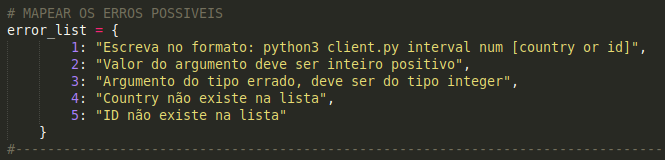
\includegraphics[width=1.1\linewidth]{error_list.png}
\caption{Error\textunderscore list}
\label{Error}
\end{figure}


\section{Função validateArgs }
\label{sec:validate}
\paragraph{}
Esta função tem como argumento o número total de argumentos introduzidos pelo utilizador e serve para validar o número de argumentos. \newline
Se forem introduzidos menos do que 4 argumentos (nome do ficheiro conta como 1 argumento), a função dá \textit{return} de 1, que é um erro mapeado. Se forem introduzidos 4 ou mais argumentos, a função dá \textit{return} de 0, que faz com que o código continue a ser executado.

\begin{figure}[H]
\centering
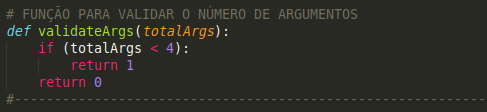
\includegraphics[width=1\linewidth]{validate_args.png}
\caption{Função validateArgs}
\label{valArgs}
\end{figure}


\section{Função isInteger }
\label{sec:isInteger}
\paragraph{}
Esta função tem como argumento um valor de qualquer tipo e verifica se esse valor é inteiro positivo. \newline 
Dentro to bloco \textit{Try} tentamos converter o valor para inteiro. Se for possível, verificamos se é maior ou igual a 0 (inteiro positivo) e, caso isto se verifique, o valor é válido, função dá \textit{return} de 0. Caso não se verifique, a função dá \textit{return} de 2, que é um erro mapeado. \newline
Se não for possível converter o número para inteiro, a função levanta uma excepção do tipo \textit{ValueError} e dá \textit{return} de 3, que é um erro mapeado.

\begin{figure}[H]
\centering
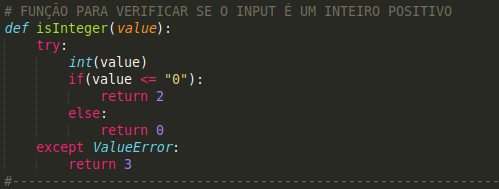
\includegraphics[width=0.8\linewidth]{integer.png}
\caption{Função isInteger}
\label{Integer}
\end{figure}


\section{Função validateIDExists }
\label{sec:valID}
\paragraph{}
Esta função tem 2 argumentos que são o ID a validar e o ficheiro em qual queremos procurar esse ID.
Vamos percorrer cada servidor do ficheiro e caso o ID de um desses servidores seja igual ao argumento ID que a função recebe, temos \textit{return} de 0 e o código continua a ser executado. \newline
Caso nenhum ID corresponda, a função dá \textit{return} de 5, que é um erro mapeado.

\begin{figure}[H]
\centering
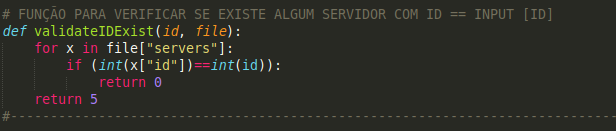
\includegraphics[width=1.1\linewidth]{valID.png}
\caption{Função validateIDExists}
\label{ID}
\end{figure}


\section{Função validateCountryExists }
\label{sec:valCountry}
\paragraph{}
Esta função tem 2 argumentos que são o país a validar e o ficheiro em qual queremos procurar esse país.
Vamos percorrer cada servidor do ficheiro e caso o país de um desses servidores seja igual ao argumento country que a função recebe, temos \textit{return} de 0 e o código continua a ser executado. \newline
Caso nenhum país corresponda, a função dá \textit{return} de 5, que é um erro mapeado.

\begin{figure}[H]
\centering
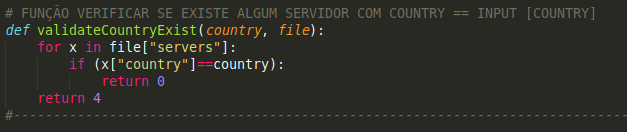
\includegraphics[width=1.1\linewidth]{valCountry.png}
\caption{Função validateCountryExists}
\label{valCount}
\end{figure}


\section{Função printError }
\label{sec:printError}
\paragraph{}
Esta função tem 1 argumento que é número do erro. Caso seja um erro mapeado, a função dá \textit{return} da respetiva mensagem associada ao número do erro.\newline
Caso não seja um erro mapeado, a função dá \textit{return} de "Unknown Error".

\begin{figure}[H]
\centering
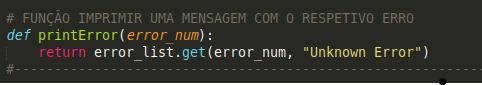
\includegraphics[width=1.1\linewidth]{printError.png}
\caption{Função printError}
\label{print}
\end{figure}

\paragraph{}

\section{Função getHostById }
\label{sec:getHostById}
\paragraph{}
Esta função tem 2 argumentos que são o ID e o ficheiro em qual queremos procurar esse ID.
Vamos percorrer cada servidor do ficheiro e caso o ID de um desses servidores seja igual ao argumento ID que a função recebe, a função dá \textit{return} do \textit{host} desse servidor.

\begin{figure}[H]
\centering
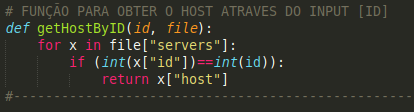
\includegraphics[width=1.1\linewidth]{getHostByID.png}
\caption{Função getHostByID}
\label{getHost}
\end{figure}


\newpage


\section{Função getHostByCountry }
\label{sec:getHostByCountry}
\paragraph{}
Esta função tem 2 argumentos que são o país a e o ficheiro em qual queremos procurar esse país.
Vamos percorrer cada servidor e caso o país desse servidor seja igual ao argumento country que a função recebe, vamos incrementar 1 à variável count (que é o número de vezes que esse país aparece). \newline
Depois vamos gerar um número aleatório de 1 até ao número de vezes que o país aparece.
Corremos todos os servidores e mais uma vez vemos quantas vezes esse país aparece, depois quando o índex for igual ao número gerado, damos \textit{return} ao \textit{host} que tenha esse índex.

\begin{figure}[H]
\centering
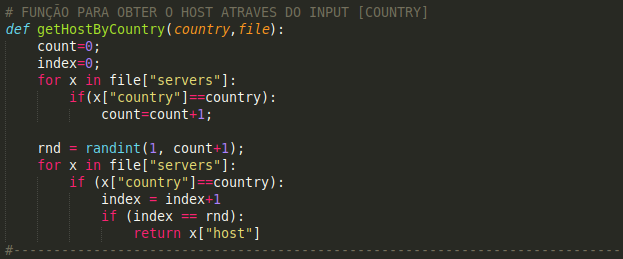
\includegraphics[width=0.9\linewidth]{getHostByCountry.png}
\caption{Função getHostByCountry}
\label{getHostCountry}
\end{figure}


\section{Função sendHi }
\label{sec:sendHi}
\paragraph{}
Esta função tem 2 argumentos que são a \textit{host} e o \textit{port} do servidor que queremos testar.
O código esta dentro de um bloco \textit{Try...Except} que nos permite apanhar as excepções mais comuns neste tipo de código. \newline
Caso o código no bloco \textit{Try} corra sem levantar excepções, a função dá \textit{return} dos dados recebidos, descodificados.
Caso ocorra uma excepção, a função dá \textit{return} de uma mensagem com o respetivo erro.

\begin{figure}[H]
\centering
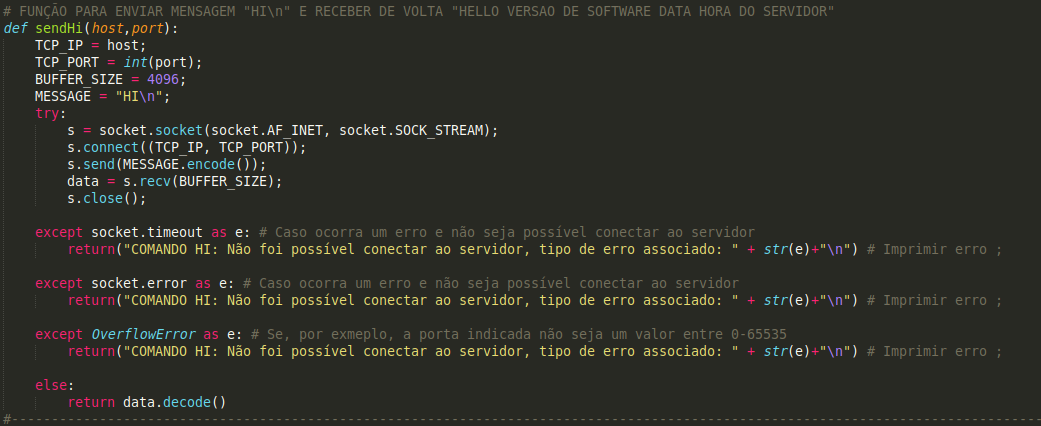
\includegraphics[width=0.9\linewidth]{sendHi.png}
\caption{Função sendHi}
\label{getIDHost}
\end{figure}


\section{Função sendPing }
\label{sec:sendPing}
\paragraph{}
Esta função tem 3 argumentos que são a \textit{host}, o \textit{port} do servidor que queremos testar e o \textit{timestamp} do momento em que mandamos a mensagem.
\paragraph{}
Dentro do bloco \textit{Try}, temos todo o código que queremos correr. Iniciamos a variável tmp\textunderscore lat\textunderscore sum fora do ciclo for pois necessitamos de incrementar valores a ela cada vez que o ciclo faça uma iteração. Obtemos a latência de cada iteração e vamos somar todos esses valores. \newline
Fora do ciclo \textit{for} dividimos esse valor de latência pelo número de iterações, neste caso 10, obtendo assim o valor médio de 10 transações PING/PONG que é a latência.
\paragraph{}
Caso ocorra uma excepção, a função dá print do erro que ocorreu e dá \textit{return} de -1.



\begin{figure}[H]
\centering
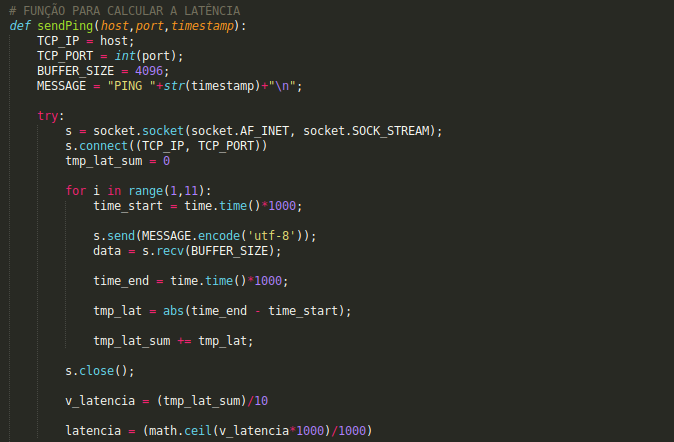
\includegraphics[width=1.2\linewidth]{sendPing1.png}
\caption{Função sendPing - Bloco Try}
\label{gePing}
\end{figure}



\begin{figure}[H]
\centering
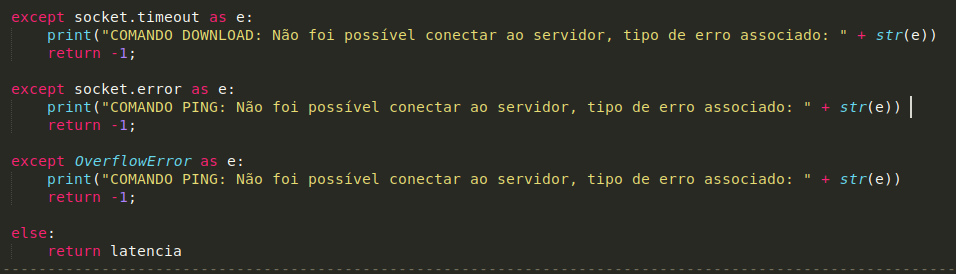
\includegraphics[width=1.2\linewidth]{sendPing2.png}
\caption{Função sendPing - Bloco das Excepções}
\label{gePing1}
\end{figure}


\newpage



\section{Função sendDownload }
\label{sec:sendDownload}
\paragraph{}
Esta função tem 2 argumentos que são a \textit{host} e o \textit{port} do servidor que queremos testar.
\paragraph{}
O tamanho do \textit{download} vai ser um inteiro aleatório entre 10000000(10MB) e 100000000(100MB). Fazemos um ciclo \textit{while} que corre enquanto não tiverem passados 10 segundos. \newline
Dentro desse ciclo temos outro ciclo \textit{while} que corre enquanto não tiverem sido feitos um \textit{download} de 1MB. Dentro deste ciclo vamos ter uma variável para contar o tempo, que vai actualizar até ter sido feito um \textit{download} de 1MB. Após isso temos o tempo em que começa, que se mantém constante.
Incrementamos o número de octetos que são baixados á medida que o ciclo \textit{while} corre.
\paragraph{}
Calculamos a largura de banda em \textit{Megabytes} por segundo e convertemos para \textit{Megabits} por segundo.
Caso ocorra uma excepção, a função dá print do erro que ocorreu e dá \textit{return} de 0.


\begin{figure}[H]
\centering
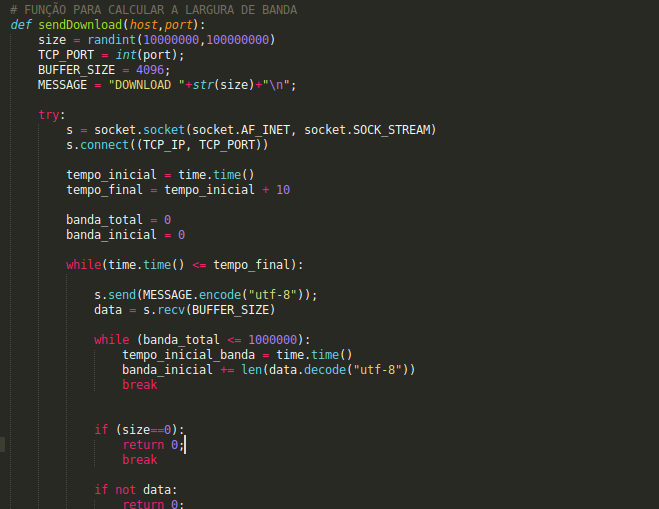
\includegraphics[width=0.9\linewidth]{sendDownload1.png}
\caption{Função sendDownload}
\label{geDown1}
\end{figure}



\begin{figure}[H]
\centering
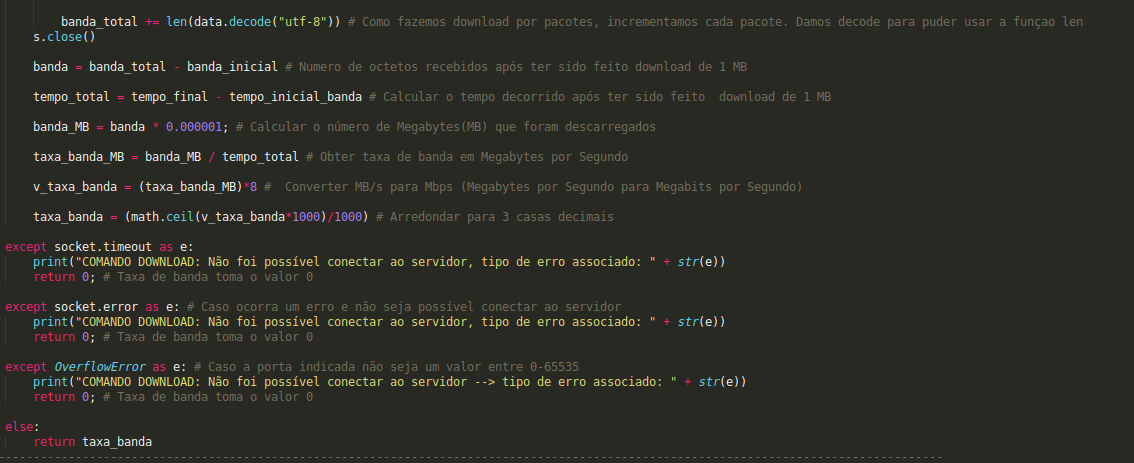
\includegraphics[width=1.2\linewidth]{sendDownload2.png}
\caption{Função sendDownload}
\label{geDown2}
\end{figure}



\section{Função getSintese }
\label{sec:getSintese}
\paragraph{}
Esta função tem 1 argumento que é o campo que queremos fazer a síntese.
Nesta função usamos a SHA3\textunderscore 512, que é das mais recentes mas também das mais seguras.
Caso ocorra uma excepção, a função da print do erro que ocorreu e o programa dá \textit{exit}.

\begin{figure}[H]
\centering
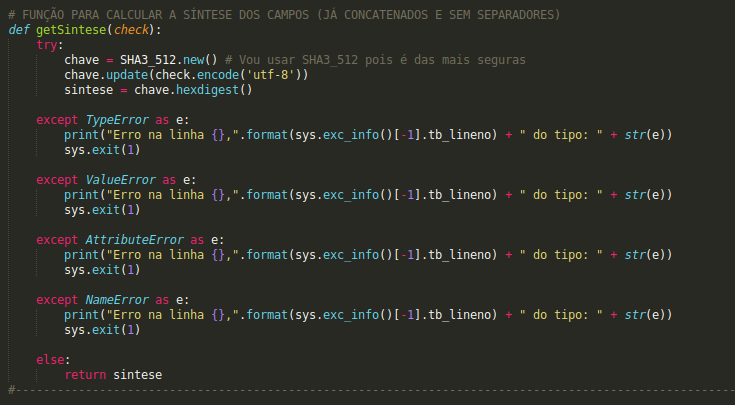
\includegraphics[width=1.1\linewidth]{getSintese.png}
\caption{Função getSintese}
\label{getSint}
\end{figure}


\section{Função getFileSintese }
\label{sec:getFileSinte}
\paragraph{}
Esta função tem 1 argumento que é o ficheiro que queremos fazer a síntese.
O buffer é cada linha do ficheiro e enquanto o ficheiro tiver linhas, vamos percorrer e fazer a síntese. \newline
Caso ocorra uma excepção, a função da print do erro que ocorreu e o programa dá \textit{exit}.

\begin{figure}[H]
\centering
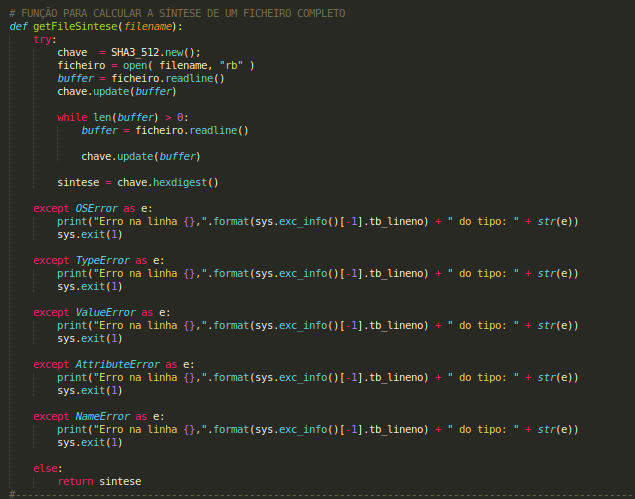
\includegraphics[width=1.1\linewidth]{getFileSintese.png}
\caption{Função getFileSintese}
\label{getFileSint}
\end{figure}


\newpage


\section{Função main }
\label{sec:main}
\paragraph{}
Esta função é a principal, que utiliza todas as funções anteriores e produz o resultado final. Devido ao tamanho, não vão haver imagens porém o código está todo comentado.
\paragraph{}
Começamos por validar todos os argumentos usando as funções necessárias, depois realizamos os testes usando um \textit{for loop}, sendo que por casa iteração, são calculadas as caracteristícas de velocidade de acesso á internet.
No fim do ciclo \textit{for}, geramos um ficheiro chamado \textbf{\textit{key.priv}}, que contém uma chave privada {\acs{rsa}}. É feita a síntese do ficheiro \textbf{\textit{report.csv}} e depois é lido o ficheiro \textbf{\textit{key.priv}}.
Usando a chave nele contida, geramos um ficheiro com a assinatura do ficheiro \textbf{\textit{report.csv}}.


\begin{figure}[H]
\centering
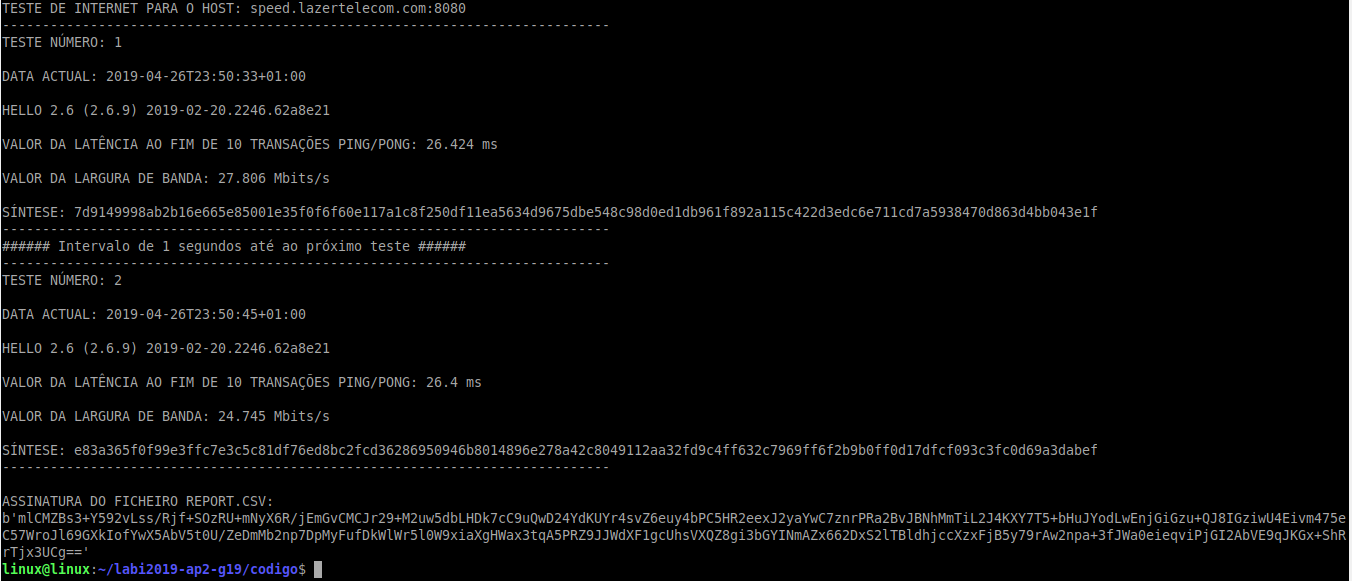
\includegraphics[width=1.3\linewidth]{main.png}
\caption{Função main após ser corrida}
\label{getFileSint}
\end{figure}


\newpage


\chapter{Implementação de testes unitários - test\textunderscore unitario\textunderscore funcoes.py}
\label{chap.Implementacao testes}
\paragraph{}
Neste capítulo vai ser uma breve exposição dos testes unitários das funções.
As funções que não estão testadas são as \textbf{\textit{sendHi}}, \textbf{\textit{sendPing}} e \textbf{\textit{sendDownload}} pois os seus resultados dependem de muitas variáveis que não podem ser controladas.
\paragraph{}
O código está todo comentado, pelo que a sua leitura é fácil.
Os testes são realizados de modo a verificar que as funções dão os resultados esperados, que dão, como podemos ver pela seguinte imagem.


\begin{figure}[H]
\centering
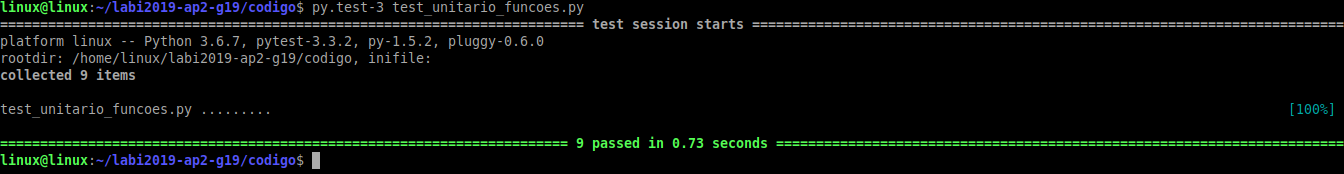
\includegraphics[width=1.3\linewidth]{testes.png}
\caption{Testes das funções}
\label{getFileSint}
\end{figure}


\newpage


\chapter{Conclusão:}
\label{chap:conclusao}
\paragraph{}	
Vivemos num mundo dominado pela \textit{internet}, é uma ferramenta que usamos todos os dias, quer seja para trabalho ou para lazer.
\paragraph{}
Com este trabalho, é possível agora ter uma ideia de como a velocidade de acesso à \textit{internet} é definida e quais os vários aspetos a ter em conta quando escolhemos um pacote de \textit{internet}. É possível também observar, pelo uso da aplicação, que a distância e o local onde o servidor está, em relação à nossa posição, tem influência na velocidade de acesso.
Espero que com este trabalho, as pessoas percebam um pouco melhor de como a \textit{internet} funciona.

\section{Contribuição dos autores}
\paragraph{}
O aluno Luís Couto ficou encarregue da realização de todo o código e do relatório.
\paragraph{}
Tendo isto em conta, a contribuição de LC foi 100\%.

%%%%%%%%%%%%%%%ACABA

\printbibliography

\end{document}


